\documentclass[a4paper,12pt]{article}

% Pacotes básicos
\usepackage{fontspec}
\setmainfont{Latin Modern Roman}

\usepackage{polyglossia}
\setmainlanguage{portuguese}

\usepackage{graphicx}
\usepackage{geometry}
\usepackage{amsmath}
\usepackage{hyperref}
\usepackage{float}
\usepackage{caption}
\usepackage{subcaption}
\usepackage{listings}
\usepackage{xcolor}
\usepackage{setspace}
\usepackage{tabularx}
\usepackage{booktabs}
% Configuração das margens
\geometry{top=3cm,bottom=2cm,left=3cm,right=2cm}

% Comando para adicionar a Fonte nas figuras (Padrão ABNT)
\newcommand{\fonte}[1]{
    \vspace{-0.2cm} \begin{center} \small \textbf{Fonte:} #1 \end{center}
}

% Configuração para códigos
\definecolor{codegreen}{rgb}{0,0.6,0}
\definecolor{codegray}{rgb}{0.5,0.5,0.5}
\definecolor{codepurple}{rgb}{0.58,0,0.82}
\definecolor{backcolour}{rgb}{0.95,0.95,0.92}

\lstdefinestyle{mystyle}{
    backgroundcolor=\color{backcolour}, commentstyle=\color{codegreen},
    keywordstyle=\color{magenta}, numberstyle=\tiny\color{codegray},
    stringstyle=\color{codepurple}, basicstyle=\ttfamily\footnotesize,
    breakatwhitespace=false, breaklines=true, captionpos=b, keepspaces=true,
    numbers=left, numbersep=5pt, showspaces=false, showstringspaces=false,
    showtabs=false, tabsize=2
}

\lstset{style=mystyle}
\title{\textbf{Relatório de Implementação de DBSCAN em MPI}}
\author{Seu Nome Aqui}
\date{Natal, \today}

\begin{document}

\begin{center}
    \thispagestyle{empty}
    
\includegraphics[scale=0.05]{Imagens/ufrn-brasao.png}

    \textbf{\large Universidade Federal do Rio Grande do Norte}\\
    \textbf{\large Sistemas Biga Data DIM0198 - 2026.2} \\
    [1cm]
    \vspace*{2cm}
    {\Huge {Relatório de Implementação de DBSCAN em MPI}}
    \\[0.5cm]
    \large Eduardo Nestor Ferreira Marinho \\
    \large Kael Amir Pina Paraguassu Silva \\
    \large Matheus Leão de Carvalho \\
    \large Samuel Morais da Rocha e Silva \\
    [1cm]
    \vfill
    \normalsize Natal, \today.
\end{center}

\newpage

\section{Implementação}

\subsection{DBScan}

A implementação do algoritmo DBSCAN foi dividida em duas fases principais: o
mapeamento de vizinhança e a expansão dos agrupamentos (\textit{clusters}).

Na primeira etapa (\texttt{calcular\_vizinhos}), o algoritmo mede a distância
euclidiana entre os pontos em $d$ dimensões e guarda quem está no $\varepsilon$ (\texttt{eps}) máximo. O próprio ponto entra na lista.
Para otimizar o processamento e facilitar a comunicação em rede, os vizinhos
identificados para cada ponto são agrupados em um único vetor contíguo na
memória (\texttt{plano}), em vez de serem armazenados em listas encadeadas
independentes. Além disso, o vetor é acompanhado por um outro vetor auxiliar que
registra a quantidade de vizinhos de cada ponto (\texttt{contagens}).

Na segunda etapa (\texttt{expandir}), os pontos são classificados a partir da
densidade de sua vizinhança. Todos os registros iniciam rotulados como ruído
(\texttt{-1}). O algoritmo então percorre a base em busca de pontos centrais, os
que têm ao menos \texttt{min\_pts} vizinhos nessa lista. Sempre que acha um
ponto central ainda sem rótulo, abre um agrupamento e o expande em largura:
vizinho de ponto central entra no grupo e, se também for central, a busca
continua a partir dele.

\subsection{Distribuição}

Como a busca de vizinhos compara cada ponto com toda a base, o MPI divide essa
carga em fatias. Todos os processos calculam a sua parte, inclusive o de
\textit{rank} 0:

\begin{enumerate}
    \item \textbf{Leitura e Difusão (\textit{Broadcast}):} O processo de
          \textit{rank} 0 carrega o arquivo binário com a matriz normalizada e
          envia as dimensões e a matriz inteira aos demais com
          \texttt{MPI\_Bcast}. %
    \item \textbf{Particionamento e Busca Paralela:} O conjunto total de $n$
          pontos é dividido de forma balanceada em fatias contíguas entre os
          processos disponíveis. Cada processo calcula, de maneira independente
          e sem necessidade de comunicação intermediária, as listas de vizinhos
          apenas para os pontos pertencentes à sua fatia local.
    \item \textbf{Consolidação (\textit{Gather}):} Os processos trocam o tamanho
          das listas (\texttt{MPI\_Allgather}) e devolvem as contagens e os
          vizinhos ao processo 0 com \texttt{MPI\_Gatherv}.
    \item \textbf{Expansão Sequencial:} Com as listas reunidas, só o processo 0
          executa \texttt{expandir}. O resultado não depende do número de
          processos, porque essa etapa é sempre a mesma.
\end{enumerate}

O monitoramento de desempenho é realizado com barreiras de sincronização
(\texttt{MPI\_Barrier}) e cronometragem (\texttt{MPI\_Wtime}), isolando os
tempos gastos na busca paralela (consolidado pelo maior tempo entre os processos
via \texttt{MPI\_Reduce}), na junção dos dados pela rede e na expansão final.

\subsection{Job}
\label{subsec:job}

Os testes de desempenho e escalabilidade foram automatizados no gerenciador de
filas Slurm por meio do script \texttt{job\_dbscan.sh}. O ambiente de execução
foi dimensionado na partição \texttt{intel-128} com a alocação de 16 nós
computacionais e até 32 tarefas por nó (1 CPU por tarefa), totalizando até 512
processos simultâneos e tempo limite de 30 minutos.

A bateria experimental executou o algoritmo sobre o arquivo
\texttt{dados/amostra.bin} utilizando os parâmetros fixos
$\varepsilon = 0{,}035$ e $\text{MinPts} = 30$. Para avaliar o comportamento do
código em diferentes escalas de paralelismo, o número de processos ($P$) foi
variado em potências de dois ($1, 2, 4, 8, 16, 32, 64, 128, 256$ e $512$),
realizando-se 3 repetições consecutivas para cada configuração a fim de obter as
médias.

\subsection{Saídas}

Ao término de cada execução, o processo mestre consolida as métricas e gera os
artefatos de saída na pasta \texttt{resultados/}: %

\begin{itemize}
    \item \textbf{Métricas de Desempenho (\texttt{tempos.csv}):} Arquivo tabular
          incrementado a cada execução com o número de processos, o índice da
          repetição, o tempo total, os tempos parciais de cada etapa (busca,
          junção e expansão) e os totais de agrupamentos e pontos de ruído.
    \item \textbf{Rótulos de Agrupamento (\texttt{rotulos\_p<nprocs>.bin}):}
          Arquivo binário contendo o vetor de classes atribuídas a cada um dos
          $n$ pontos da amostra, utilizado posteriormente pelos scripts de
          visualização.
    \item \textbf{Resumo da Execução (\texttt{resumo.json}):} Gerado na execução
          de referência com 1 processo, documenta os hiperparâmetros utilizados,
          a quantidade de agrupamentos e ruídos encontrados e o tamanho dos 10
          maiores \textit{clusters}.
\end{itemize}

\section{Resultados}

\subsection{Desempenho}

\subsubsection{Eficiência, \textit{speedup} e tempos de execução}

A tabela pura produzida em formato CSV foi agregada com o objetivo de resumir as
métricas de tempo de execução em relação às três execuções para cada
configuração de número de processos. O resultado é uma tabela com os seguintes
atributos:

\begin{itemize}
    \item $N_p$ (Índice): O número de processos paralelos utilizados na execução
          do algoritmo.
    \item $\bar{T}_{total}$: O tempo médio total decorrido para a execução
          completa do algoritmo considerando as repetições (em segundos).
    \item $\bar{T}_{buscar}$: A média do maior tempo gasto na etapa de busca de
          vizinhos dentro do algoritmo (em segundos). Utilizamos o maior tempo
          para a operação de busca entre os nós por este ser o gargalo da
          execução distribuída.
    \item $\bar{T}_{gather}$: O tempo médio gasto no processo de consolidação de
          dados paralelos (operação \textit{gather}) (em segundos).
    \item $\bar{T}_{expandir}$: O tempo médio gasto especificamente na expansão
          dos clusters paralelos (em segundos).
\end{itemize}

A Tabela~\ref{tab:desempenho_processos} consolida os resultados obtidos.

\begin{table}[h]
    \centering
    \caption{Métricas médias de desempenho por número de processos paralelo.}
    \label{tab:desempenho_processos}
    \begin{tabular}{lcccccc}
        \toprule
        & $\bar{T}_{total}$ & $\bar{T}_{buscar}$ & $\bar{T}_{gather}$ &
        $\bar{T}_{expandir}$ \\
        \
        $N_p$ & & & & & & \\
        \midrule
        1 & 1.4196 & 1.4107 & 0.0049 & 0.0039 \\
        2 & 0.6940 & 0.6839 & 0.0052 & 0.0043 \\
        4 & 0.3575 & 0.3454 & 0.0070 & 0.0037 \\
        8 & 0.2034 & 0.1889 & 0.0084 & 0.0037 \\
        16 & 0.1143 & 0.0954 & 0.0117 & 0.0039 \\
        32 & 0.1457 & 0.1015 & 0.0175 & 0.0056 \\
        64 & 0.1334 & 0.0542 & 0.0362 & 0.0060 \\
        128 & 0.1498 & 0.0293 & 0.0448 & 0.0062 \\
        256 & 1.1404 & 0.0162 & 1.1115 & 0.0060 \\
        512 & 1.1314 & 0.0085 & 0.9416 & 0.0064 \\
        \bottomrule
    \end{tabular}
\end{table}

Para uma análise mais aprofundada, foram calculados os valores de
\textit{speedup} e eficiência médios, tomando como base os valores de
$\bar{T}_{total}$ para as diferentes configurações de números de processos.

As valores da análise estão visíveis na Tabela~\ref{tab:speedup}, e organizados
graficamente na

\begin{table}
    \centering
    \caption{
        \textit{Speedup} e Eficiência médias obtidas para o tempo total de
        execução.
    }
    \label{tab:speedup}
    \begin{tabular}{lcc}
        \toprule
        $N_p$ & $\bar{S}$ & $\bar{E}$ \\
        1     &  1.0000   &  1.0000   \\
        2     &  2.0455   &  1.0227   \\
        4     &  3.9709   &  0.9927   \\
        8     &  6.9798   &  0.8725   \\
        16    &  12.4208  &  0.7763   \\
        32    &  9.7427   &  0.3045   \\
        64    &  10.6404  &  0.1663   \\
        128   &  9.4779   &  0.0740   \\
        256   &  1.2448   &  0.0049   \\
        512   &  1.2547   &  0.0025   \\
        \bottomrule
    \end{tabular}
\end{table}

\begin{figure}[h]
    \centering
    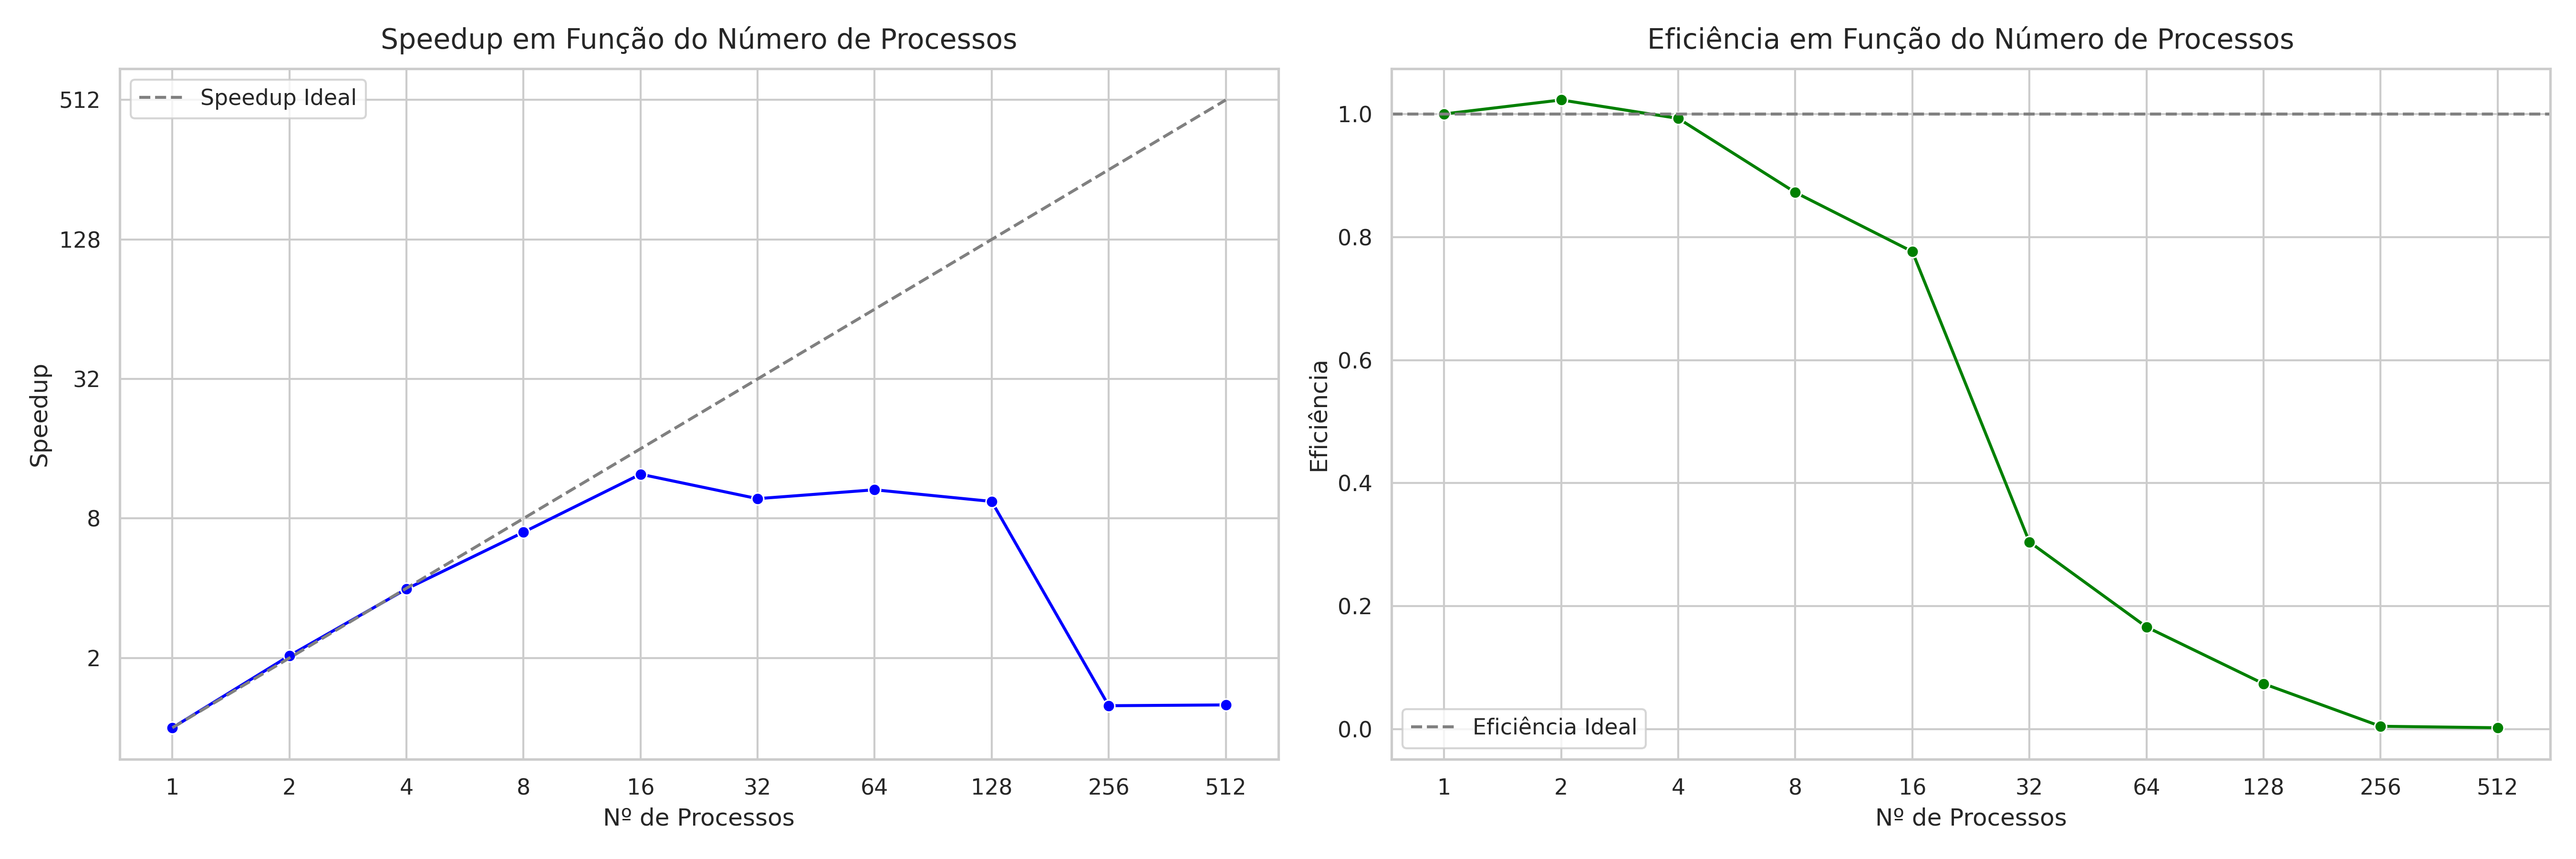
\includegraphics[width=1.0\linewidth]{Imagens/graficos_speedup_eficiencia.png}
    \caption{\textsf{Gráficos de \textit{speedup} e eficiência médios.}}
    \label{fig:grafico}
\end{figure}

De posse da agregação, foi construído um gráfico de linhas da
Figura~\ref{fig:grafico} detalhando, para cada número de processos, o tempo
médio total da execução da rotina e das operações que a compõe.

\begin{figure}[h]
    \centering
    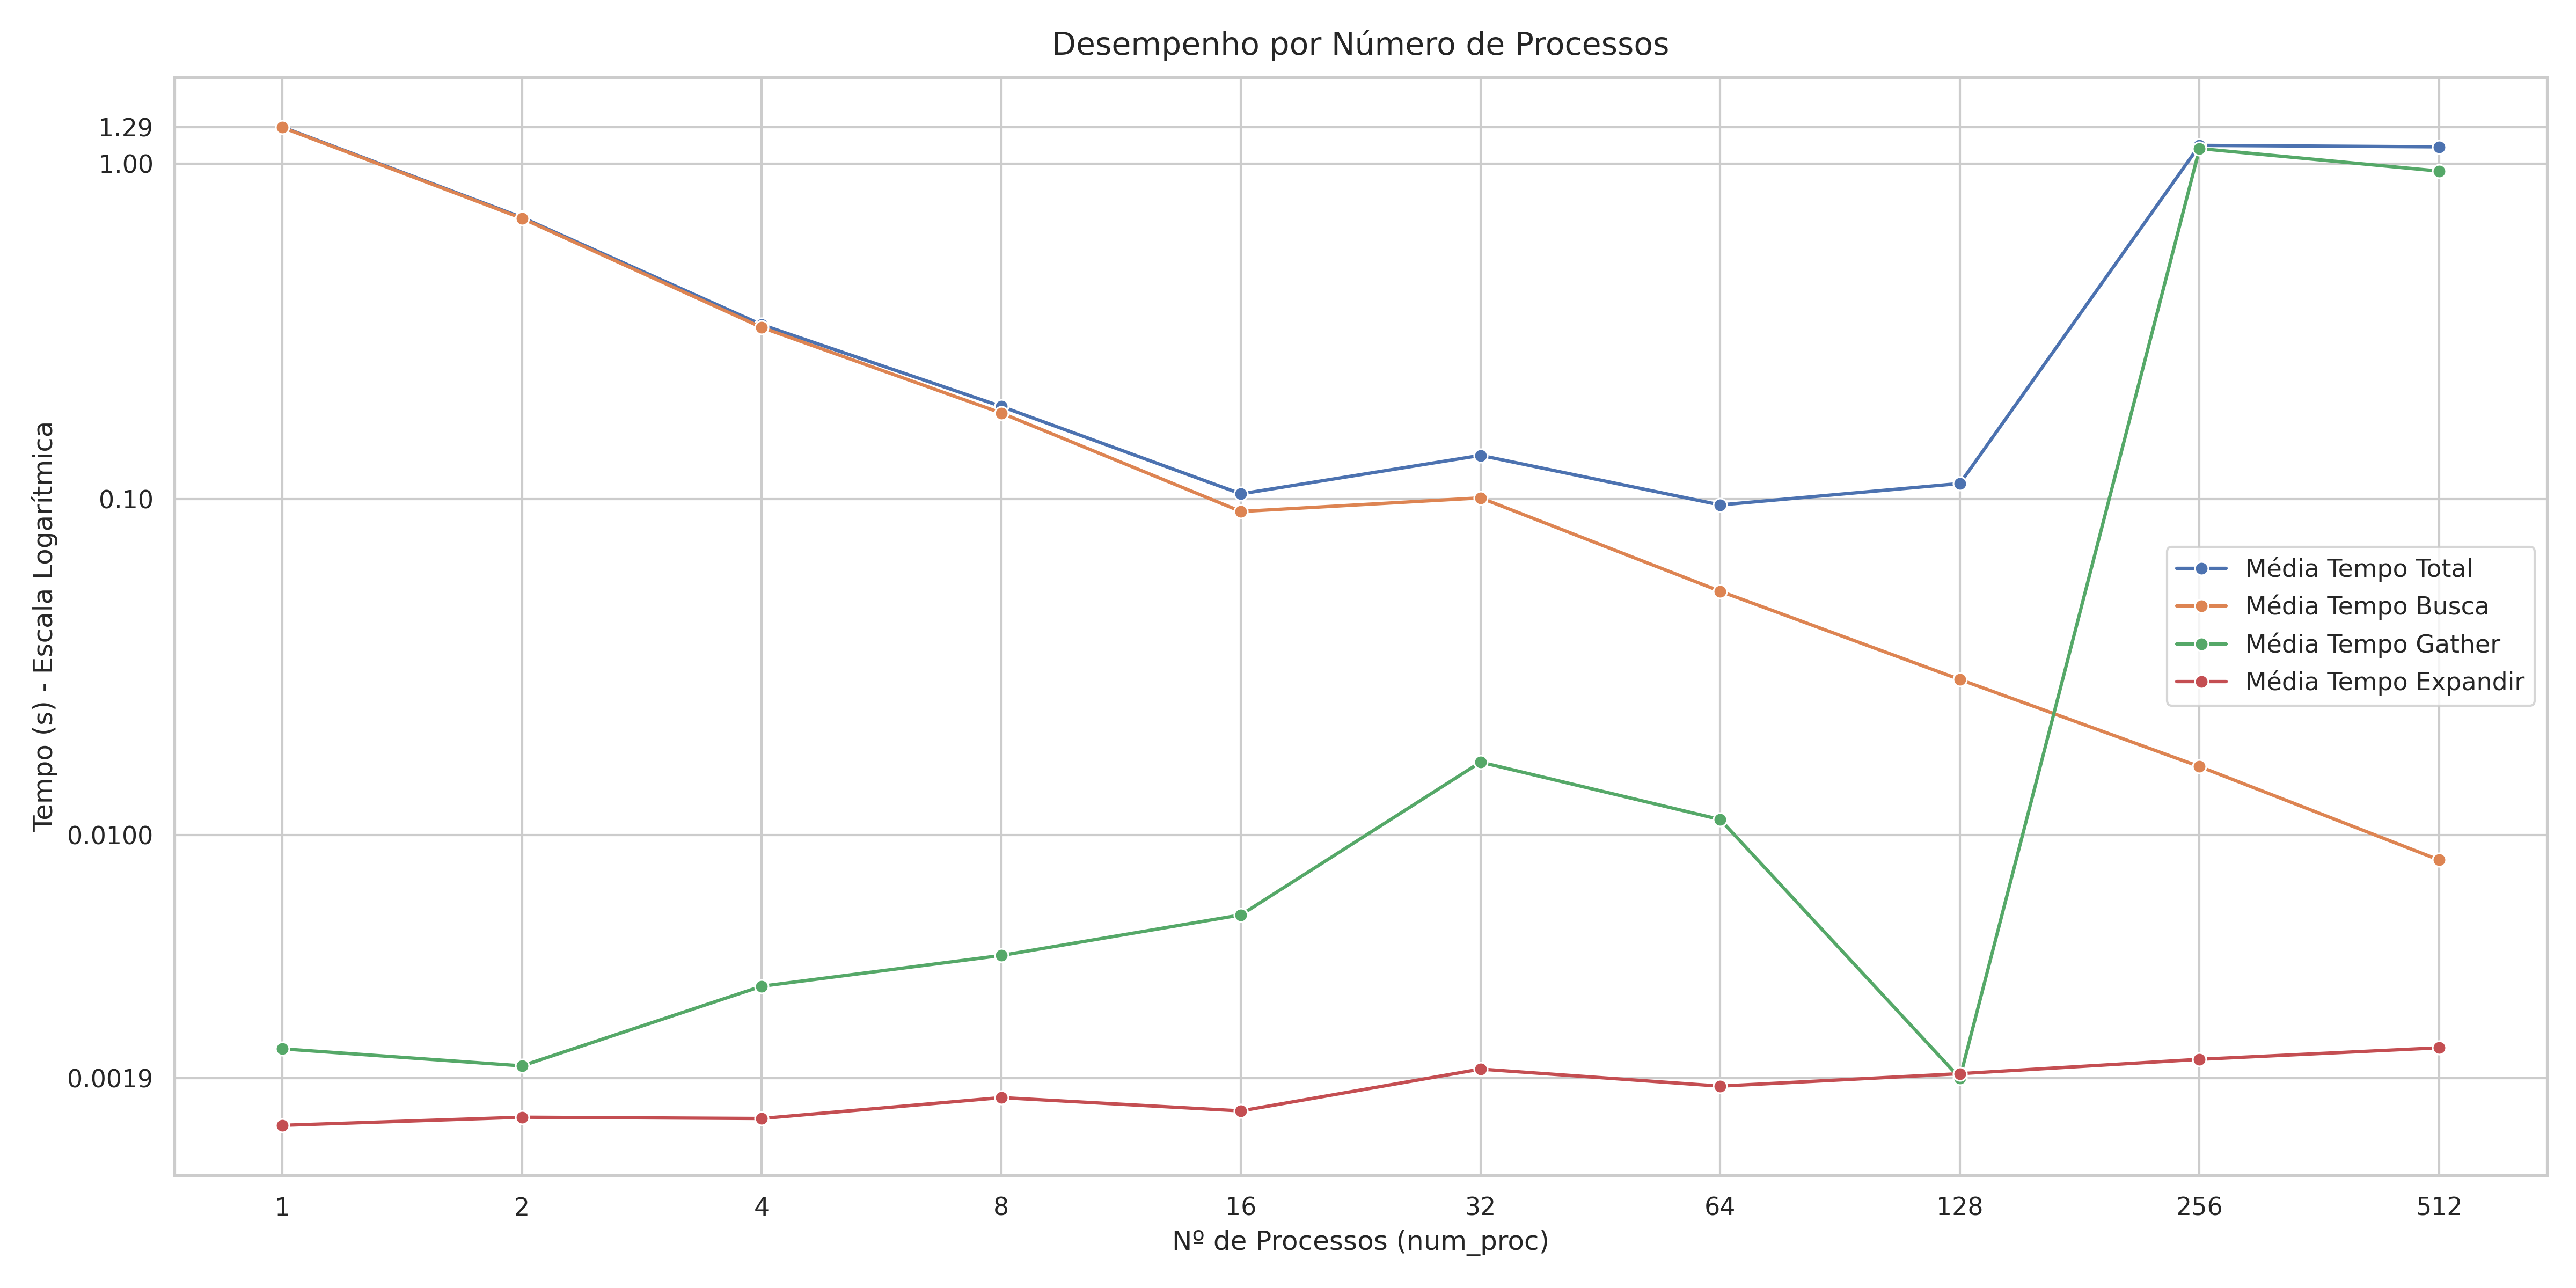
\includegraphics[width=1.0\linewidth]{Imagens/graficos_desempenho.png}
    \caption{\textsf{Gráfico de tempo de execução do DBScan.}}
    \label{fig:grafico}
\end{figure}

Dentre pontos de observação valiosos do gráfico, destacam-se:
\begin{itemize}
    \item O salto no tempo decorrido para a operação de \textit{gather} mediante
          o aumento de 128 a 256 processos. O salto é justificado pelo uso da
          partição \texttt{Intel-128} para a execução do \textit{job}: sua
          limitação de 128 núcleos faz com que a partir deste ponto, a
          comunicação entre nós computacionais distintos seja inevitável. Essa
          dominância da latência de rede sobre o tempo de execução é expressado
          pelo aumento no tempo dedicado à operação \textit{gather}.
    \item O tempo decorrido para a operação de busca decai de forma quase linear
          com a proliferação dos processos. Isso ocorre pois esta operação é
          \textbf{local}, não envolvendo trocas de mensagem na rede. Ou seja,
          esta operação beneficia-se grandemente pelo processamento distribuído,
          já que a quantidade de pontos processados em cada instância reduz com
          a adição de processos, diminuindo, também, o esforço de cada
          processador.
\end{itemize}

\newpage

\subsection{\textit{Clustering}}

\begin{figure}[h]
    \centering
    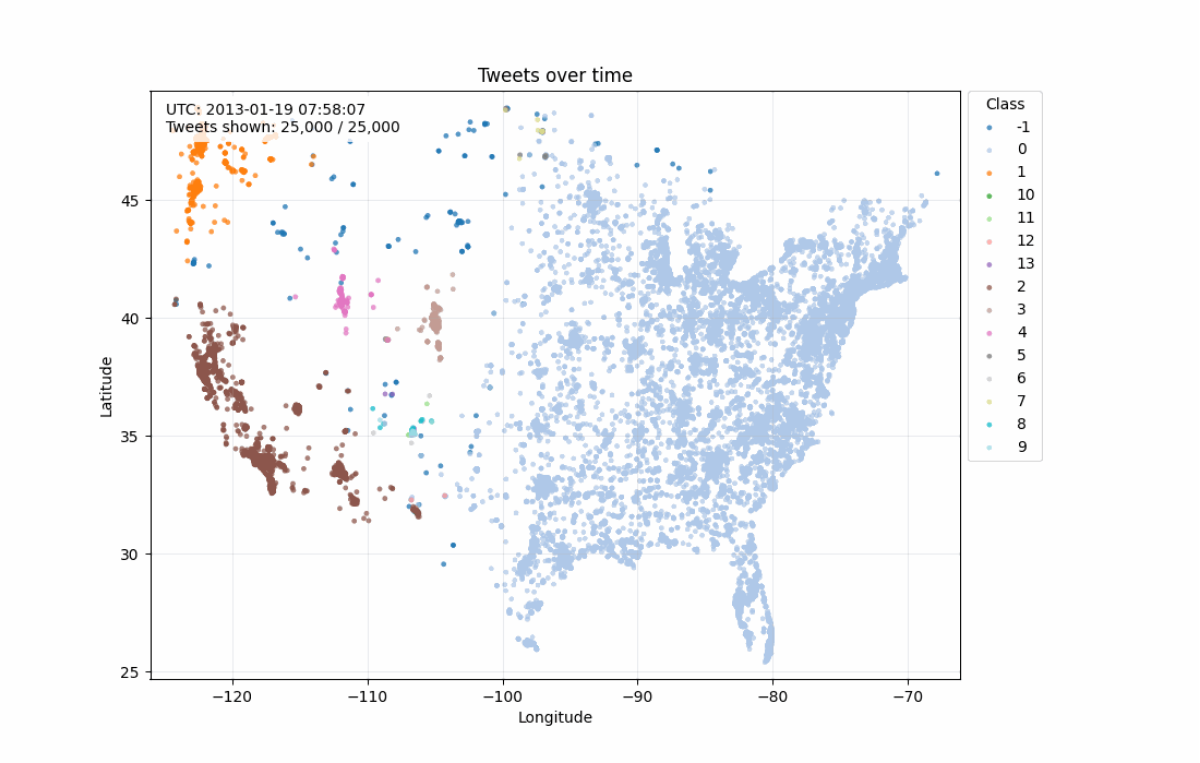
\includegraphics[width=1.1\linewidth]{Imagens/clustering.png}
    \caption{\textsf{Exemplo de clustering.}}
    \label{fig:clustering}
\end{figure}

\end{document}
